\section{Does the Evidence Call for More Precision?}
\label{sec:sameprec}

\begin{figure*}[t]
\begin{minipage}[t]{\columnwidth}
\centering
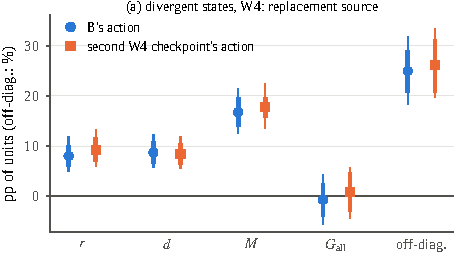
\includegraphics[width=\columnwidth]{figures/f6a_sameprec_rates.pdf}
\end{minipage}\hfill
\begin{minipage}[t]{\columnwidth}
\centering
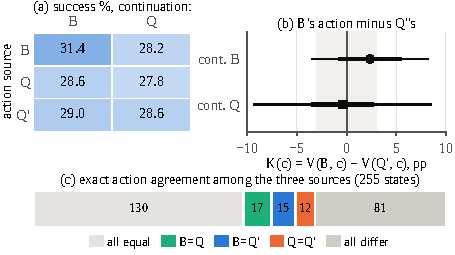
\includegraphics[width=\columnwidth]{figures/f8_commonstate.pdf}
\end{minipage}
\caption{Does an upgrade need a higher bit width? (a)~Each design at its own first divergence, W4 (q4 and q8 GPTQ-W4 pooled; 1020 units; $n_{\mathrm{blk}}=6$): replacing Q's action with B's (circles) or with a second W4 checkpoint's (squares); rescues $r$, damages $d$, turnover $M$ and net $\Gall$ in pp of units, off-diagonal share in \% of divergent states; thick: fixed-pool 95\% ($t$ over block means), thin: new-task 95\% (crossed). (b--d)~Common states (q8; 510 pre-registered ordinary states, 6 blocks): (b)~success (\%) by action source and continuation; (c)~$K(c)$, B's action value beyond a second W4 checkpoint's; here, unlike (a), thick: task-cluster bootstrap 95\%, thin: $t$ (block means) 95\%; shaded: $\pm$3\pp{}; (d)~exact agreement of the three actions. Overlap of affected units, equivalence tests, per-model numbers and two-look intervals: Appendix~\ref{app:sameprec}.} % src: analysis/fork/out/sameprec_20261004T070601Z.json; analysis/fork/out/sameprec_20261004T070601Z.md (analysis set K = 6); analysis/fork/out/commonstate_q8ext_20261003T231159Z.json; analysis/fork/out/commonstate_q8ext_20261003T231159Z.md; paper/latex/figures/provenance.json (f6a_sameprec_rates, f8_commonstate)
\label{fig:sameprec}
\label{fig:commonstate}
\end{figure*}

A large turnover or a frequent interaction might suggest that a state needs higher precision. If these consequences required a higher bit width, the same-precision substitution (\S\ref{sec:estimands}) should produce markedly fewer of them. Its protocol was frozen before any outcome; the common-state comparison is pre-registered; the overlap analyses are descriptive. Each design forks at its own first divergence, so the two may select different states. We therefore cannot read flips found by only one design as caused by precision, or flips found by both as not caused by it.

\paragraph{A higher bit width is not necessary for two-sided flips and continuation dependence.} They also appear when only the calibration checkpoint is swapped (Figure~\ref{fig:sameprec}a). At W4 (frozen final analysis set, $n_{\mathrm{blk}}=6$), the second checkpoint's action rescues $r'=9.3$ (fixed pool [7.0, 11.7]; new tasks [5.9, 13.2]) and damages $d'=8.4$ ([6.4, 10.5]; [5.5, 12.0])\pp{} of units ($M'=17.7$\% against $M=16.8$\% for B on the same 6 blocks and two GPTQ-W4 configurations; Table~\ref{tab:refs}), and 26.2\% of its divergent states are off the diagonal, against 25.0\% for B; each same-precision rate has a fixed-pool 95\% lower bound above zero. % src: docs/insights/SAMEPREC_PROTOCOL.md (A1.3, 95% lower bound); analysis/fork/out/sameprec_20261004T070601Z.md (TL;DR; Full pool; On divergent states; analysis set K = 6); analysis/fork/out/sameprec_20261004T070601Z.json (pooled.same.rescue/damage.crossed_ci95)
In the W3 stress pair the turnovers are 17.3\% (second W3 checkpoint) and 18.8\% (B) and the off-diagonal shares 27.6\% and 27.3\%. Flip rate and interaction size alone therefore cannot diagnose a need for a higher bit width. We do not claim the turnovers are equal: neither pair is equivalent within $\pm$3\pp{} (Appendix~\ref{app:sameprec}). % src: analysis/fork/out/sameprec_w3_20261004T070607Z.md (TL;DR; Full pool, pool rows)

\paragraph{Units affected by both, or by only one, substitution.} At W4 (Appendix~\ref{app:sameprec}), 107 units flip under both substitutions, 64 only under B and 74 only under the second checkpoint. A within-task block shuffle, which keeps each task's flip propensity, gives 76 [69, 84] units flipping under both, so the two substitutions share affected units beyond what flip-prone tasks explain. % src: analysis/fork/out/sameprec_overlap_20261002T143218Z.md (Overlap table; Agreement); analysis/fork/out/sameprec_w3_split_20261003T024007Z.md (Figure-panel table, G rows)
The overlap lies in action replacement: over the 1020 W4 units, Cohen's $\kappa$ between the indicators ``B's action rescues'' and ``the second checkpoint's action rescues'' is $\kappa_r=0.60$, and for damages $\kappa_d=0.54$. When B also takes over the continuation, the affected units are largely substitution-specific (Appendix~\ref{app:sameprec}). The difference in action-side net value ($\Delta\Gall$) comes only from the substitution-specific units and is not resolved ($-1.6$\pp{}; fixed pool [$-6.2$, $+3.0$], new tasks [$-6.5$, $+3.6$]). % src: analysis/fork/out/sameprec_split_20261002T145148Z.md (TL;DR; Figure-panel table; §1; §2; §3); analysis/fork/out/sameprec_20261004T070601Z.json (pooled.paired.dG.crossed_ci95)

\paragraph{Common states.} A pre-registered comparison holds the states fixed: on 510 ordinary q8 states (85 tasks $\times$ 6 blocks), the current action comes from B, from Q or from a second W4 checkpoint Q$'$, and B or Q continues (Figure~\ref{fig:commonstate}b--d). Under Q's continuation, replacing Q's action by B's flips 7.1\% of outcomes for a net $+1.2$\pp{}; replacing it by Q$'$'s flips 8.0\% for a net $+0.2$\pp{}. What B's action adds beyond another W4 action, $K(c)=V(\mathrm{B},c)-V(\mathrm{Q}',c)$, is $+1.0$\pp{} under Q's continuation and $+0.8$\pp{} under B's. After the fixed extension from three to six blocks, no advantage is resolved (95\% $t$ [$-3.5$, $+5.4$] and [$-1.8$, $+3.3$]). Under B's continuation the ordinary 90\% interval lies within $\pm$3\pp{} (two one-sided tests, $t$ [$-1.2$, $+2.8$]), but the two-look sensitivity analysis (94\% intervals) does not, so we do not claim equivalence; q4 (two blocks) is also not resolved (Appendix~\ref{app:sameprec}). Replacing Q's action with Q$'$'s under Q's continuation is within $\pm$3\pp{} of no change by the same tests (descriptive). Sensitivity to an action, the value higher precision adds at a state, and the gain of a given upgrade thus need separate measurements. % src: docs/insights/COMMONSTATE_SOURCES_PROTOCOL.md (§2, §5, §6; A1.1, A1.3; D2.2); analysis/fork/out/commonstate_q8ext_20261003T231159Z.md (TL;DR; Contrasts table: bf16 − d1 and d2 − d1 at c = d1, columns Δ and M, reading; Key estimand table, t95 and t90; Two-look reading table); analysis/fork/out/commonstate_q4_20261004T001159Z.md (TL;DR, q4 K)


